% !TEX TS-program = pdflatex
% !TEX encoding = UTF-8 Unicode

% This is a simple template for a LaTeX document using the "article" class.
% See "book", "report", "letter" for other types of document.

\documentclass[11pt]{article} % use larger type; default would be 10pt

\usepackage[utf8]{inputenc} % set input encoding (not needed with XeLaTeX)

%%% PAGE DIMENSIONS
\usepackage{geometry} % to change the page dimensions
\geometry{a4paper} % or letterpaper (US) or a5paper or....

\usepackage{graphicx} % support the \includegraphics command and options

\usepackage{amssymb}
\usepackage{amsmath}
%%% PACKAGES
\usepackage{booktabs} % for much better looking tables
\usepackage{array} % for better arrays (eg matrices) in maths
\usepackage{paralist} % very flexible & customisable lists (eg. enumerate/itemize, etc.)
\usepackage{verbatim} % adds environment for commenting out blocks of text & for better verbatim
\usepackage{subfig} % make it possible to include more than one captioned figure/table in a single float
% These packages are all incorporated in the memoir class to one degree or another...

%%% HEADERS & FOOTERS
\usepackage{fancyhdr} % This should be set AFTER setting up the page geometry
\pagestyle{fancy} % options: empty , plain , fancy
\renewcommand{\headrulewidth}{0pt} % customise the layout...
\lhead{}\chead{}\rhead{}
\lfoot{}\cfoot{\thepage}\rfoot{}

%%% SECTION TITLE APPEARANCE
\usepackage{sectsty}
\allsectionsfont{\sffamily\mdseries\upshape} % (See the fntguide.pdf for font help)
% (This matches ConTeXt defaults)

%%% ToC (table of contents) APPEARANCE
\usepackage[nottoc,notlof,notlot]{tocbibind} % Put the bibliography in the ToC
\usepackage[titles,subfigure]{tocloft} % Alter the style of the Table of Contents
\renewcommand{\cftsecfont}{\rmfamily\mdseries\upshape}
\renewcommand{\cftsecpagefont}{\rmfamily\mdseries\upshape} % No bold!
\usepackage{graphicx}
\graphicspath{ {./pings/} }

\usepackage{amsmath}
\DeclareMathOperator*{\argmax}{arg\,max}
\DeclareMathOperator*{\argmin}{arg\,min}

\newcount\colveccount
\newcommand*\colvec[1]{
        \global\colveccount#1
        \begin{pmatrix}
        \colvecnext
}
\def\colvecnext#1{
        #1
        \global\advance\colveccount-1
        \ifnum\colveccount>0
                \\
                \expandafter\colvecnext
        \else
                \end{pmatrix}
        \fi
}

%%% END Article customizations

%%% The "real" document content comes below...

\title{Macro PS1}
\author{Michael B. Nattinger\footnote{I worked on this assignment with my study group: Alex von Hafften, Andrew Smith, and Ryan Mather. I have also discussed problem(s) with Emily Case, Sarah Bass, Katherine Kwok, and Danny Edgel.}}

%\date{} % Activate to display a given date or no date (if empty),
         % otherwise the current date is printed 

\begin{document}
\maketitle
\section{Question 1}
The social planner maximizes the agent's utility subject to the resource constraint. 
\begin{align*}
\max_{\{C_t,K_{t+1}\} }\sum_{t=0}^{\infty} \beta^t U(C_t)\\
\text{s.t. } F(K_t) = C_t + I_t
\end{align*}
 We can solve our law of motion for capital for $I_t$ and write our lagrangian as follows:
\begin{align*}
\mathcal{L} &= \sum_{t=0}^{\infty} \beta^t U(C_t) + \lambda_t(F(K_t) - C_t + (1-\delta)K_t - K_{t+1} - D_t).
\end{align*}

We solve for our Euler equation by taking first order conditions with respect to consumption and capital:
\begin{align*}
\beta^t U'(C_t) &= \lambda_t\\
\lambda_{t+1} (F'(K_{t+1}) + 1-\delta) &= \lambda_t \\
\Rightarrow U'(C_t) &= \beta U'(C_{t+1}) (F'(K_{t+1}) + 1-\delta).
\end{align*}

We combine our euler equation with the law of motion of capital along with our transversality condition to define the solution to the planner's problem:
\begin{align}
U'(C_t) &= \beta U'(C_{t+1}) (F'(K_{t+1}) + 1-\delta), \label{euler}\\
K_{t+1} &= (1-\delta) K_t + F(K_t) - C_t - D_t \label{lomk}\\
\lim_{t\rightarrow \infty} \beta^t U'(C_{t}) K_{t+1} &= 0. \label{tvc}
\end{align}

\section{Question 2}
Given $D$, we can use (\ref{euler}), (\ref{lomk}) to solve for $\bar{K}(D),\bar{C}(D)$ as follows:
\begin{align*}
1 &= \beta  (F'(\bar{K}(D)) + 1-\delta)\\
\Rightarrow \bar{K}(D)&= (F')^{-1}\left(\frac{1}{\beta} -1 +\delta\right),\\
\bar{C}(D) &= F(\bar{K}(D)) - \delta\bar{K}(D) - D.
\end{align*}

We can find the curves for the phase diagram by setting $\Delta K = 0, \Delta C = 0:$
\begin{align*}
\Delta C = 0 &\Rightarrow 1 = \beta  (F'(K) + 1-\delta)\\
\Delta K = 0 &\Rightarrow C = F(K) -\delta K - D.
\end{align*}

The phase diagram is plotted below, drawn in Matlab using the specifications detailed in question (4) of this problem set. Saddle path is calculated using the shooting method.

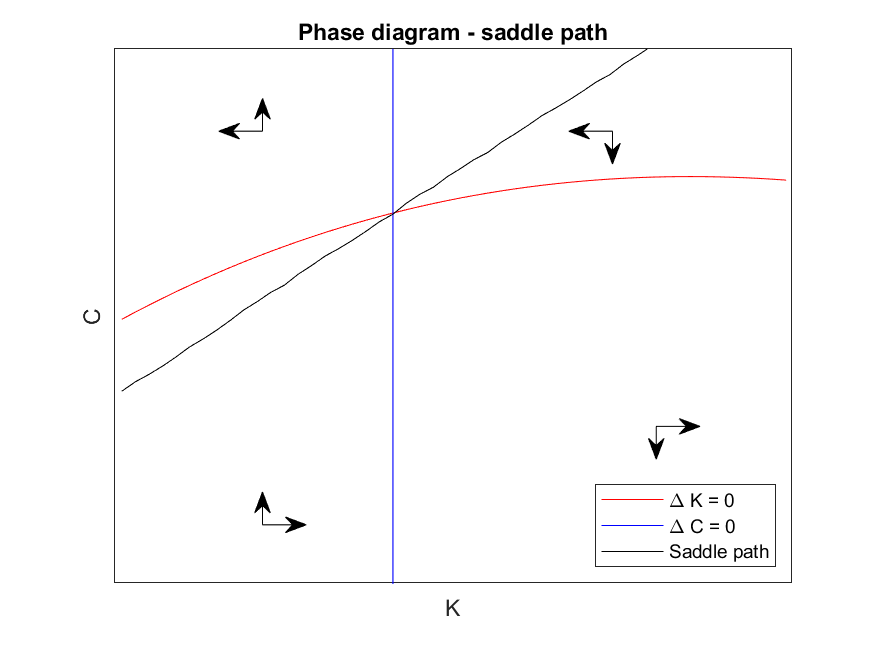
\includegraphics{phasesad}

The above figure shows the curves defining $\Delta K = 0$ and $\Delta C = 0$, the saddle path, and arrows representing the direction of change. Below I plot the zoomed-out phase diagram that shows all three steady states.

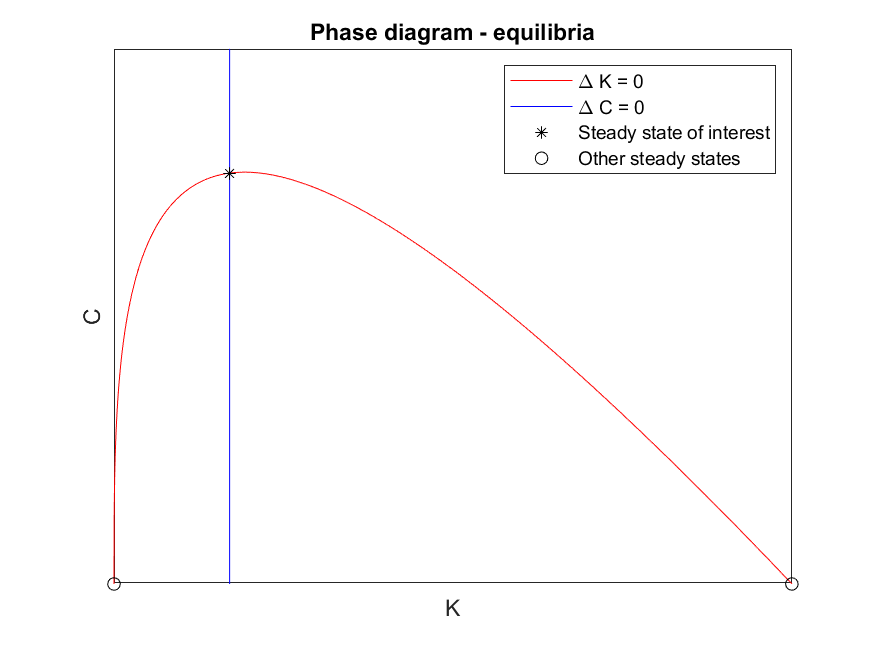
\includegraphics{phaseeq}

The above figure shows all three steady states. The main steady state is at the intersection of the curves defining $\Delta K = 0$ and $\Delta C = 0$. The other two equilibria are at the intersection of the curve defining $\Delta K = 0$ and the x-axis. 

\section{Question 3}
The control variable will adjust such that at time T the economy is on the saddle path. As the earthquake is temporary, the earthquake has no long-term impact. In other words, the steady state of the economy before and after the shock are the same. However, there is a temporary transition. At the time of the news, the agents anticipate the shock, which will negatively affect capital at time T, and to offset this the agents will consume less and save more in the short run to build up capital in anticipation of the earthquake. Then, after the earthquake, the economy will be on the saddle path and will eventually return to the steady state.

Note that it cannot be the case that consumption will increase at the time of the news. Say this were to occur. Then, the economy would proceed over the next T periods up and to the left of the steady state. When the earthquake hits, the economy would have already been to the left of the saddle path, and would be pushed further left by the earthquake. Therefore, the economy cannot end up on the saddle path if consumption increases at the time of the earthquake news. Consumption must therefore fall at the time of the news, so that immediately before the news the economy is to the right of the saddle path, and then the earthquake will push the economy to the left and onto the saddle path.

Below, I plot the transition of the economy in a phase diagram. At the time of the news, the agents reduce their consumption to invest in capital to offset the earthquake. So, consumption immediately falls, and over the next T-1 periods capital rises. At time T, capital falls due to the earthquake, and the economy ends up on the saddle path. It then follows the saddle path up and to the right until it eventually converges back to the steady state in the limit as $t\rightarrow \infty.$

 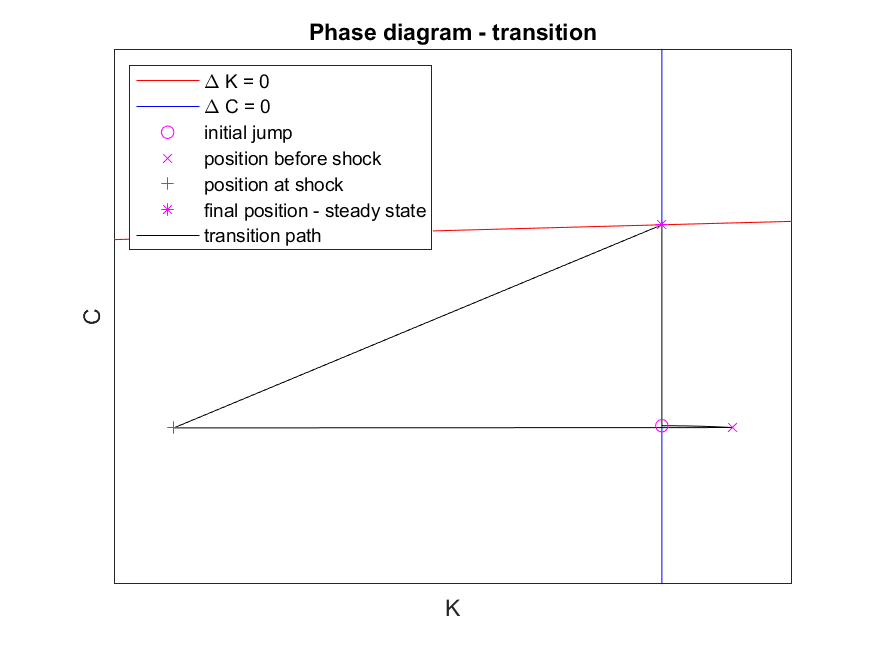
\includegraphics{phtrnolab}

The above figure shows the transition of the economy via a phase diagram, as described above. Below we show the transition of the economy in the short-run and the long-run transition to the steady state.

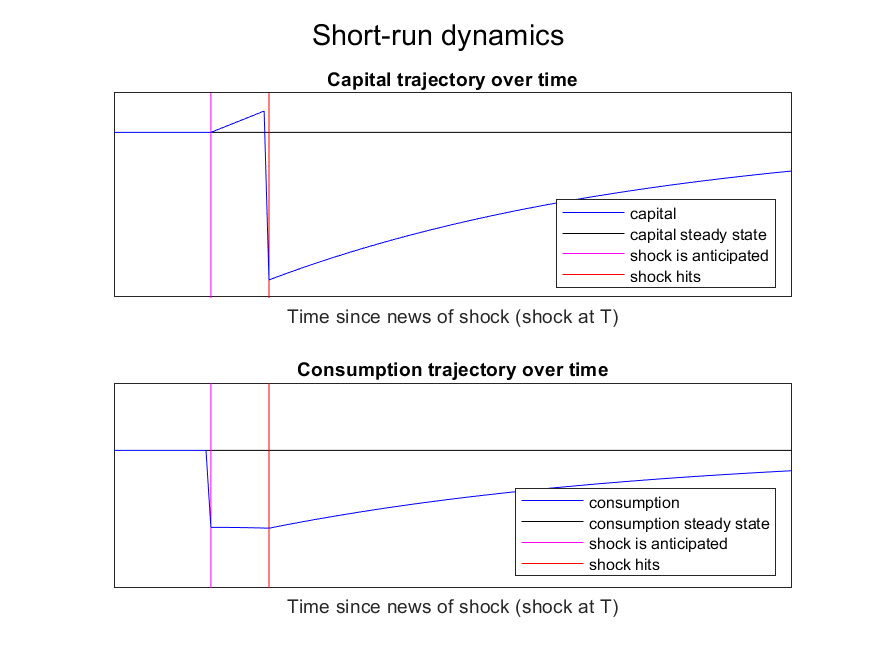
\includegraphics{shortrunnolab}

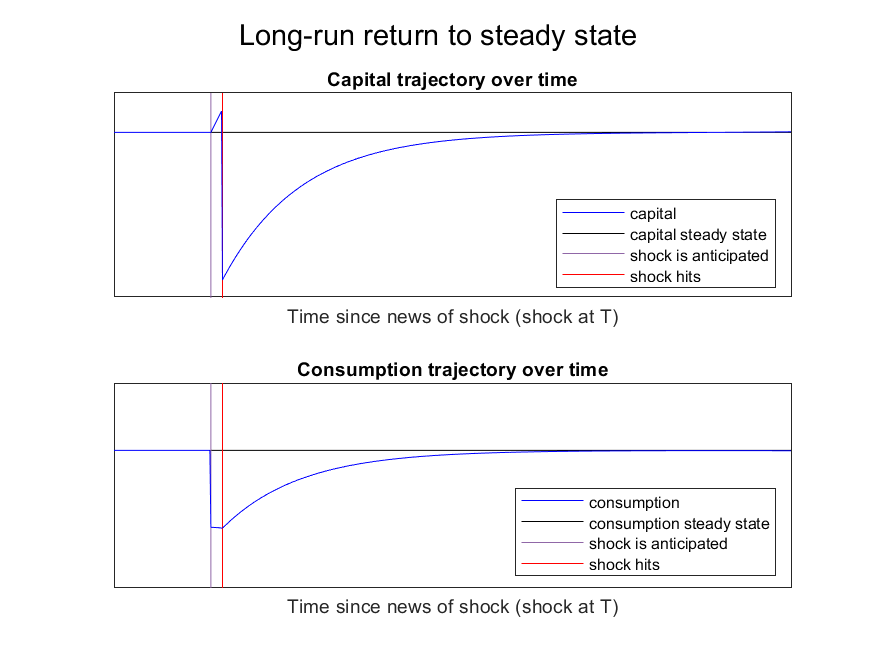
\includegraphics{longrunnolab}

\section{Question 4}

Below I plot the numerical solutions. Our results match the predictions from theory described in Question 3. That is, at the time of the announcement, the agents reduce their consumption to invest more. This increases the capital stock, until the earthquake hits. After the earthquake, the economy is on the saddle path, upon which it proceeds towards the steady state.

 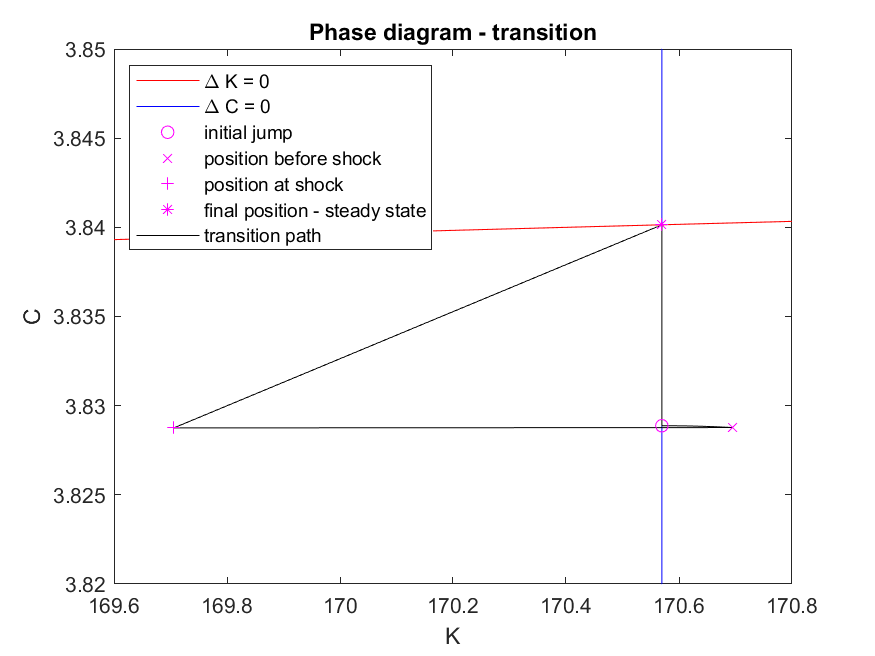
\includegraphics{phtr}

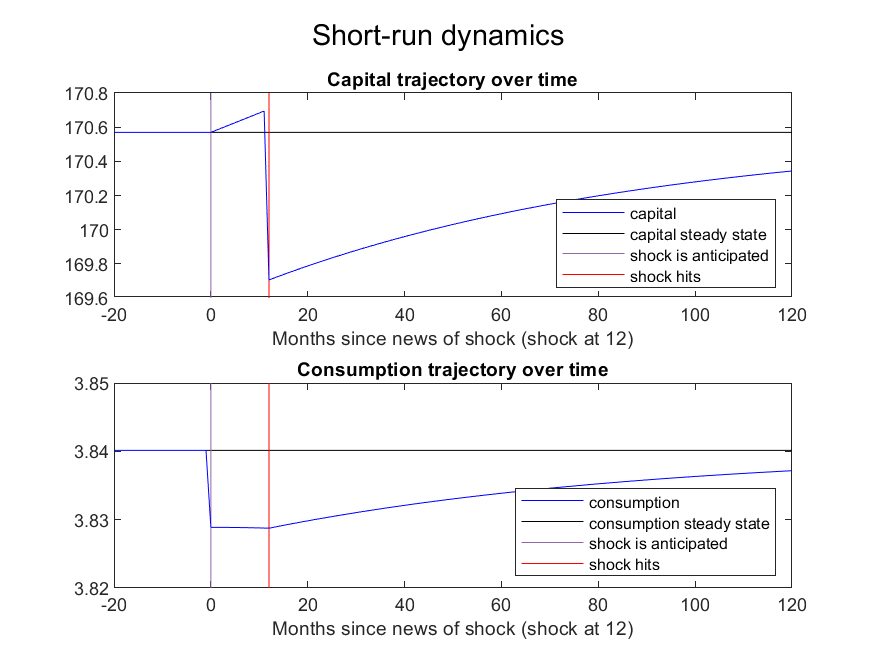
\includegraphics{shortrun}

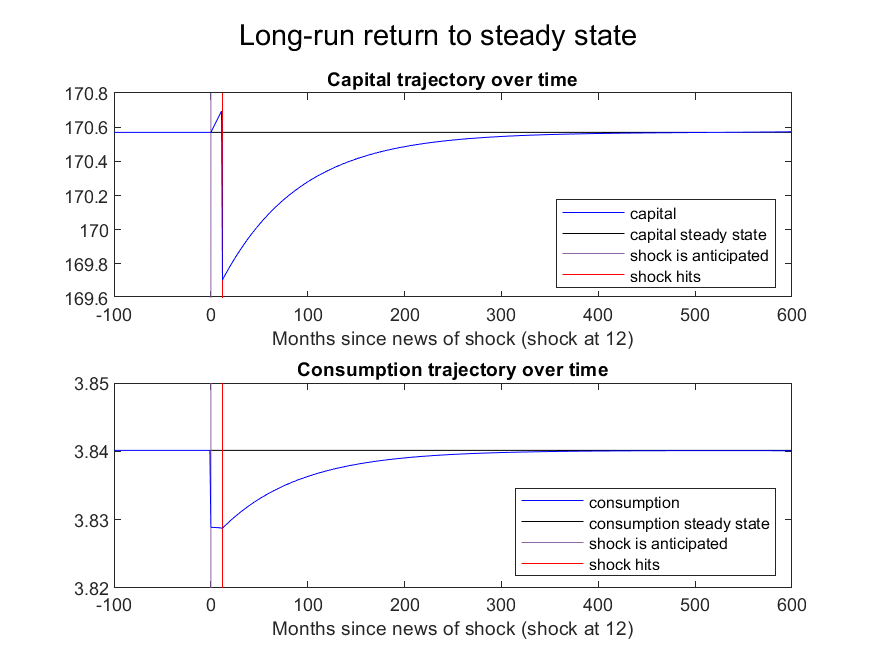
\includegraphics{longrun}

\end{document}
